% !TeX root = ../main.tex
\chapter{对极几何}
通过上一章的介绍,我们知道了如何在一张图中的提取出特征点和对应的描述子,并通过描述子的匹配来获取两张图片特征点的对应关系。在上一章的最后我们提到了基础矩阵和单应矩阵,它们都属于对极几何的范畴,这一章就来介绍一下对极几何。
\section{对极约束}
立体成像的基本几何就是对极几何。图\ref{epipolargeometry}是最经典的对极几何示意图。$O_1$和$O_2$为两个相机(也有可能是一个相机在不同时刻的位置)的位置,P为空间中一点,两个相对的白色平面是归一化平面。$p_1$和$p_2$是P点在归一化平面上的对应点,$e_1$,$e_2$为归一化平面和$O_1$,$O_2$的交点。$O_1$$O_2$为基线,也被称作相机的移动方向。\par
\begin{figure}[H]
	\centering
	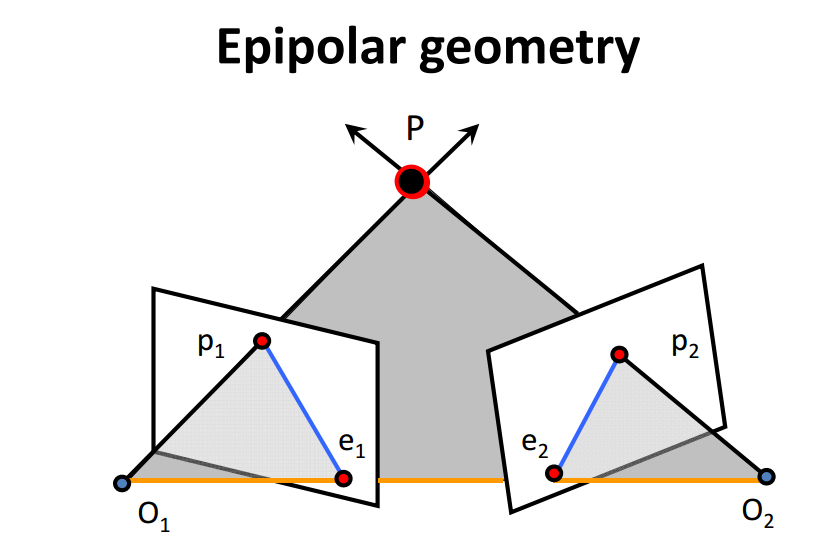
\includegraphics[height=5cm]{epipolargeometry}
	\caption{对极几何}
	\label{epipolargeometry}
\end{figure}
这里介绍几个对极几何中常用的概念: $e_1$和$e_2$被称作极点,P$O_1$$O_2$平面为极面,$p_1$$e_1$为极线,同理$p_2$$e_2$也为极线。
所谓对极约束,指的就是相机$O_1,O_2,\text{点}P$在同一个平面上。也就是向量$\overrightarrow{O_1O_2},\overrightarrow{O_1P},\overrightarrow{O_2P}$共面,即三者混合积为0:
\begin{equation}
\overrightarrow{O_1P}\cdot\left[\overrightarrow{O_1O_2}\times\overrightarrow{O_2P} \right]=0
\end{equation}
设相机$O_2$相对于相机$O_1$的旋转为R,位移为t,向量$\overrightarrow{O_1p_1}$为$\vec{x}$($O_1$坐标系下),向量$\overrightarrow{O_2p_2}$为$\vec{x^\prime}$($O_2$坐标系下),两相机的内参是$K_1,K_2$,由相机成像原理知:
\begin{equation}
\begin{aligned}
	d_{1} \boldsymbol{x}_{1}=&\boldsymbol{K}_{1} \boldsymbol{P}\\
	d_{2} \boldsymbol{x}_{2}=&\boldsymbol{K}_{2}(\boldsymbol{R P}+\boldsymbol{t})
\end{aligned}
\end{equation}
联立上式得:
\begin{equation}
d_{2} \boldsymbol{K}_{2}^{-1} \boldsymbol{x}_{2}=d_{1}\boldsymbol{R} \boldsymbol{K}_{1}^{-1} \boldsymbol{x}_{1}+\boldsymbol{t}
\end{equation}
两边同时叉乘t\footnote{$\mathbf{a} \times \mathbf{b}=\left[ \begin{array}{ccc}{0} & {-a_{z}} & {a_{y}} \\ {a_{z}} & {0} & {-a_{x}} \\ {-a_{y}} & {a_{x}} & {0}\end{array}\right] \left[ \begin{array}{l}{b_{x}} \\ {b_{y}} \\ {b_{z}}\end{array}\right]=\left[ \mathbf{a}\right]_{\times}\mathbf{b}$}:
\begin{equation}
d_{2} \left[\boldsymbol{t}\right]_{\times}\boldsymbol{K}_{2}^{-1} \boldsymbol{x}_{2}=d_{1}\left[\boldsymbol{t}\right]_{\times}\boldsymbol{R} \boldsymbol{K}_{1}^{-1} \boldsymbol{x}_{1}
\end{equation}
再同时左乘$\left(\boldsymbol{K}_{2}^{-1} \boldsymbol{x}_{2}\right)^T$:
\begin{equation}
\boldsymbol{x}_{2}^T\boldsymbol{K}_{2}^{-T} \left[\boldsymbol{t}\right]_{\times}\boldsymbol{R} \boldsymbol{K}_{1}^{-1} \boldsymbol{x}_{1}=0
\end{equation}
若令$\boldsymbol{K}_{1}^{-1} \boldsymbol{x}_{1}=\hat{\boldsymbol{x}}_1,\boldsymbol{K}_{2}^{-1} \boldsymbol{x}_{2}=\hat{\boldsymbol{x}}_2$,也就是$\hat{\boldsymbol{x}}_1,\hat{\boldsymbol{x}}_2$分别为归一化平面坐标,则:
\begin{equation}
\hat{\boldsymbol{x}}_2^T\left[\boldsymbol{t}\right]_{\times}\boldsymbol{R}\hat{\boldsymbol{x}}_1=0
\end{equation}
我们称本质矩阵$\boldsymbol{E}=[\boldsymbol{t}]_{\times} \boldsymbol{R}$,基础矩阵$\boldsymbol{F}=\boldsymbol{K}_{2}^{-T} \boldsymbol{E} \boldsymbol{K}_{1}^{-1}$\par
\section{基础矩阵}
可以看到,我们之所以要求解本质矩阵或者基础矩阵,是因为它们包含着图像之间的运动信息,只要求得本质矩阵,就能够从中分解除R和t,那么相机的运动信息也就清楚了。想要求解本质矩阵,首先要求解基础矩阵,然后去掉内参信息就能得到本质矩阵。求解基础矩阵我们一般有以下方法。
\subsection{直接线性变换法}
对于一对匹配点$\boldsymbol{x}_{1}=\left[ u_{1},v_{1},1\right]^{\mathrm{T}}, \boldsymbol{x}_{2}=\left[ u_{2},v_{2},1\right]^{\mathrm{T}}$根据对极约束$\boldsymbol{x}_{2}^{T} \boldsymbol{F x}_{1}=\mathbf{0}$:
\begin{equation}
\left( \begin{array}{ccc}{u_{1}} & {v_{1}} & {1}\end{array}\right) \left[ \begin{array}{ccc}{F_{11}} & {F_{12}} & {F_{13}} \\ {F_{21}} & {F_{22}} & {F_{23}} \\ {F_{31}} & {F_{32}} & {F_{33}}\end{array}\right] \left( \begin{array}{l}{u_{2}} \\ {v_{2}} \\ {1}\end{array}\right)=0
\end{equation}
令$f=\left[ F_{11},F_{12},F_{13},F_{21},F_{22},F_{23},F_{31},F_{32},F_{33} \right]^{T}$则有:
\begin{equation}
\left[
{u_{1} u_{1},}{u_{1} v_{2},}{u_{1},}{v_{2} u_{1},}{v_{1} v_{2},}{v_{1},}{u_{2},}{v_{2},}{1}
\right] f=0
\end{equation}
当有n对匹配点时:
\begin{equation}
\boldsymbol{A}=
\left\lbrace
	\begin{array}{c}
	u_{1}^{(1)} u_{1}^{(1)}, u_{1}^{(1)} v_{2}^{(1)}, u_{1}^{(1)},  v_{1}^{(1)} u_{2}^{(1)}, v_{1}^{(1)} v_{2}^{(1)}, v_{1}^{(1)}, u_{2}^{(1)}, v_{2}^{(1)},1\\
	u_{1}^{(2)} u_{1}^{(2)}, u_{1}^{(2)} v_{2}^{(2)}, u_{1}^{(2)},  v_{1}^{(2)} u_{2}^{(2)}, v_{1}^{(2)} v_{2}^{(2)}, v_{1}^{(2)}, u_{2}^{(2)}, v_{2}^{(2)},1\\
	\cdots\\
	u_{1}^{(n)} u_{1}^{(n)}, u_{1}^{(n)} v_{2}^{(n)}, u_{1}^{(n)},  v_{1}^{(n)} u_{2}^{(n)}, v_{1}^{(n)} v_{2}^{(n)}, v_{1}^{(n)}, u_{2}^{(n)}, v_{2}^{(n)},1\\
	\end{array}
\right\rbrace 
\end{equation}
即$\boldsymbol{A}f=0$。
要保证有唯一解至少需要8对匹配点,当匹配点n=8时,若A非奇异,则有唯一解,称为8点法\cite{longuet1981computer}。若n>8,则可用最小二乘解,也就是$\boldsymbol{A}^T\boldsymbol{A}$的最小特征值对应的特征向量即为最优解。
\subsection{RANSAC法}
RANSAC方法的思想我们在上一章已经介绍过了,应用RANSAC法求解基础矩阵也是有以下几个步骤:
\begin{enumerate}
	\item 随机从匹配的点对中选择8个点,使用8点法估算出基础矩阵$F_i$
	\item 计算其余的点对到其对应对极线的距离$d_n$,如果$d_n≤d$则该点为内点,否则为外点。记下符合该条件的内点的个数为$m_i$
	\item 迭代k次,或者某次得到内点的数目$m_i$占有的比例大于等于95\%,则停止。选择$m_i$最大的基础矩阵作为最终的结果。
\end{enumerate}\par
RANSAC能够不依赖于任何额外信息的情况下,将数据划分为内点和外点。但也有其相应的缺点,RANSAC并不能保证得到正确的结果,需要提高迭代的次数;另一个是,内点外点的判断需要设置阈值。\par
阈值的大小设置也是有技巧的,对于不同图片大小,需要设置不同的阈值。事实上经过实验,采用归一化平面坐标而不是像素坐标来计算基础矩阵会有较好的结果。
\section{单应矩阵}
除了基础矩阵和本质矩阵,还有单应矩阵(Homography)$\boldsymbol{H}$,它主要适用于特征点都位于同一个平面上的情况。比如两个相机都拍摄一面纹理丰富的墙,这就是单应矩阵大展身手的时候。下面我们来大概介绍一下单应矩阵\par
\begin{figure}[H]
	\centering
	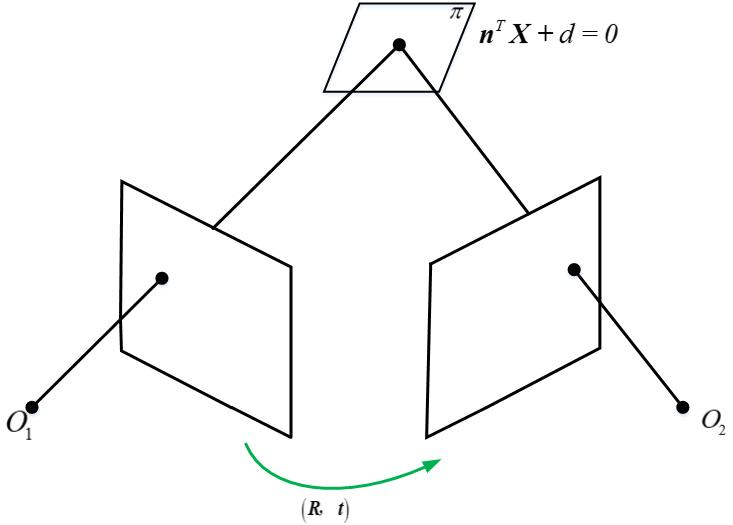
\includegraphics[height=5cm]{homography}
	\caption{单应矩阵条件}
\end{figure}
设特征点所在的平面方程为:
\begin{equation}
	\boldsymbol{n}^{T} \boldsymbol{P}+d=0 \Rightarrow -\frac{\boldsymbol{n}^{T} \boldsymbol{P}}{d}=1
\end{equation}
故:
\begin{equation}
\begin{aligned} x_{2} &=K_{2}(R P+t) \\ &=K_{2}\left(R P+t \cdot\left(-\frac{n^{T} P}{d}\right)\right) \\ &=K_{2}\left(R-\frac{t n^{T}}{d}\right) P \\ &=K_{2}\left(R-\frac{t n^{T}}{d}\right) K_{1}^{-1} x_{1} \end{aligned}
\end{equation}
故:
\begin{equation}
\boldsymbol{x}_{2}=\boldsymbol{H x}_{1}, \quad \boldsymbol{H}=\boldsymbol{K}_{2}\left(\boldsymbol{R}-\frac{\boldsymbol{t} \boldsymbol{n}^{T}}{d}\right) \boldsymbol{K}_{1}^{-1}
\label{homography}
\end{equation}
单应矩阵说明了两个成像平面像素之间的映射关系,从公式\ref{homography}上来看,单应矩阵只和空间平面位置$\boldsymbol{n}$,旋转矩阵R,平移t以及相机内参有关。由于单应矩阵的平面假设,我们常在拍摄对象在平面场景时或者可以假设近似为平面场景时(如无人机俯拍)应用单应矩阵来恢复相机位姿。
\section{相机姿态的恢复}
这里介绍一下如何通过本质矩阵$E$来对相机的位姿$R,t$进行恢复。我们主要用到的方法是SVD分解\cite{multiview}。\par
首先对E进行SVD分解:
\begin{equation}
\boldsymbol{E}=\boldsymbol{U} \Sigma \boldsymbol{V}^{T}, \quad \boldsymbol{\Sigma}=\operatorname{diag}(\sigma, \quad \sigma, \quad 0)
\end{equation}
此时有两个t和两个R都有可能成立
\begin{equation}
\begin{array}{cc}
{t_{1}=U( :, 2)} & {R_{1}=U R_{Z}\left(\frac{\pi}{2}\right) V^{T}} \\
{t_{2}=-U( :, 2)} & {R_{2}=U R_{Z}^{T}\left(\frac{\pi}{2}\right) V^{T}}
\end{array}
\end{equation}
其中:
\begin{equation}
\boldsymbol{R}_{z}\left(\frac{\pi}{2}\right)=\left( \begin{array}{ccc}{0,} & {-1,} & {0} \\ {1,} & {0,} & {0} \\ {0,} & {0,} & {1}\end{array}\right), \boldsymbol{R}_{z}^{T}\left(\frac{\pi}{2}\right)=\left( \begin{array}{ccc}{0,} & {1} & {0} \\ {-1} & {0,} & {0} \\ {0,} & {0,} & {1}\end{array}\right)
\end{equation}
如下图所示,我们得到了四种情况$(t_1,R_1),(t_1,R_2),(t_2,R_1),(t_2,R_2)$。此时,我们只需要验证一下哪一种情况下点P在两个相机的正面。OpenCV已经为我们提供了方便的函数recoverpose()由本质矩阵恢复$R,t$。
\begin{figure}[H]
	\centering
	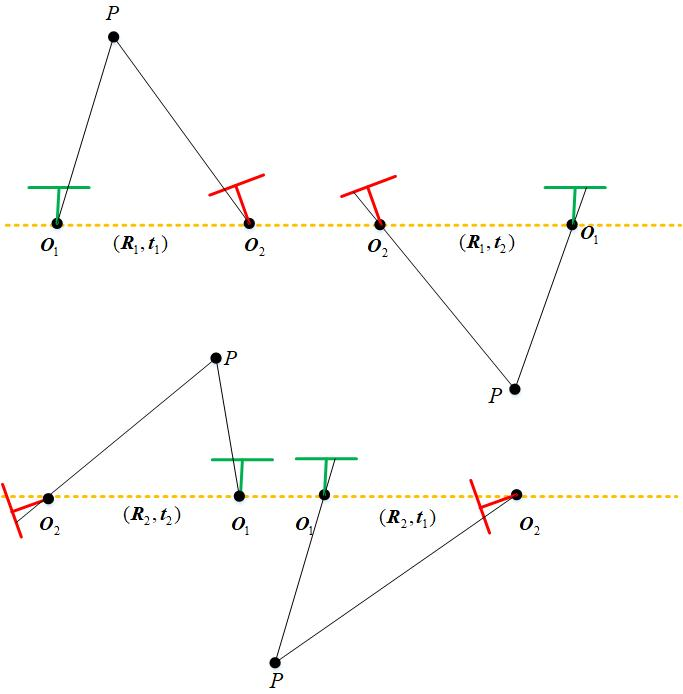
\includegraphics[height=10cm]{svd}
	\caption{四种可能的情况}
\end{figure}






















